
Soluzione dell'esercizio \ref{ex_2pca} a pagina \pageref{ex_2pca}\label{sol_2pca} \label{s_2pca}

\begin{enumerate}
\item All the forces acting on the block of mass $M_1$:

\begin{figure}[h]
\centering
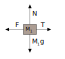
\includegraphics[width=0.4\textwidth]{carrucole.6.pdf}
\end{figure}

\begin{itemize}
\item[$M_1g$] è la \textbf{forza peso} 
\item[$N$] è la \textbf{reazione vincolare} del piano, reazione del piano stesso alla forza peso che impedisce al corpo di cadere attraverso il piano
\item[$T$] è la tensione esercitata dalla fune
\item[$F$] è la \textbf{forza d’attrito dinamico} o \textbf{statico}, a seconda che il corpo sia in quiete o in movimento.
\end{itemize}

\item 
La tensione della fune è pari alla forza esercitata dalla gravità su $M_2$:
\begin{equation*}
T=m_2g
\end{equation*}

Questo valore deve essere equivalente alla forza d'attrito dinamico:

\begin{equation*}
T=f_{max}=\mu_sm_1g
\end{equation*}

\begin{equation*}
\mu_sm_1g=m_2g
\end{equation*}

\begin{equation*}
\mu_s=\frac{m_2}{m_1}
\end{equation*}

\end{enumerate}

Soluzioni degli esercizi multiple choice da pagina \pageref{q_mcmc} \label{s_mcmc}

\begin{enumerate}
\item B
\item C
\item B
\item C
\item B
\item A
\item C
\item C
\item D
\item C
\item B
\item C
\item D
\item C
\item A
\item D
\item D
\item D
\item B
\item C
\item A
\item D
\item C
\item A, B
\item B, C
\end{enumerate}



\vspace{1cm}
\hrule
\vspace{1cm}


Soluzione dell' esercizio \ref{motocirc_e_00} a pagina \pageref{motocirc_e_00} \label{motocirc_s_00}

La risposta corretta è la ``C".

Un corpo che si muove su una traiettoria curva possiede in generale una componente
dell’accelerazione tangenziale, ossia diretta lungo la tangente alla traiettoria, responsabile
della variazione in modulo della velocità, ed una componente normale, diretta in direzione
radiale rispetto alla traiettoria e verso il centro della curva; essa è responsabile della varia-
zione in direzione della velocità. In un moto uniforme (velocità in modulo costante) la
componente tangenziale è nulla, per cui nel caso in esame è presente solo l’accelerazione
normale. 

